\chapter{Invariants and Monovariants}% by Raiyan Jamil}
\label{sec:inv-mono}

\begin{linkb}
   \begin{itemize}
        \item \href{https://www.youtube.com/watch?v=hInrF3biygw}{Invariants (Raiyan)}
        \item \href{https://drive.google.com/file/d/1Ndgs_ftSaG1Ph5sJYsIbwgGczM_NNgrW/view}{Class Note}
        \item \href{https://drive.google.com/file/d/15XjviqGWzT3T_7-W7g2axDdOXiE2le8K/view}{Invariants and Monovariants}
   \end{itemize}
\end{linkb}

This topic covers the trick of Invariant and Monovariants which are very powerful weapons to tackle hard combinatorial problems. 

Invariant means which doesn't change after some steps or operations. 

Monovariants means the value changes only in one direction, either it increases or decreases.

\section{Invariants}

\begin{example}
You have an equilateral triangle. In each "step", you can:
	\begin{itemize}
		\item Draw a line on the current shape and cut it into two pieces along the line.
		\item Then flip one of the pieces and join the two pieces again along the line.
	\end{itemize} 
\end{example}

\begin{figure}[h!]
\centering
		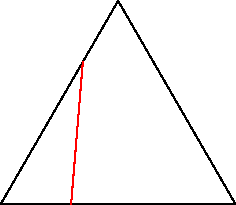
\includegraphics{equi-tri.pdf}
\end{figure}

\begin{soln}
After some move you may realize that, the perimeter and the area of the shape remains same as initial position.

SO if we want to make it a square then let the sise length of the square is $x$, and the length of the side of the equilateral triangle is $a$, so w havefollowing two equation:
\[\frac{\sqrt 3}{4}a^2 = x^2\]
\[3a = 4x.\]
which have no common solution. So it is not possible to make it a square.

\end{soln}


\begin{example}
In an empty room, in every minute either $4$ people enter or $3$ people leave. Can there be $7^{125}+5$ people in the room after $7^{666}$ minutes?
\end{example}

\begin{soln}
The trick in htis problem is to work with mod $7$, per $7$ minutes.

Let ititially there are $x$ people in the room. So in $7$ minutes there let $4$ people inter $a$ times and $7-a$ people leave the room. So after seven minutes there are $x+4a -3(7-a)=x+7(a-3)$ people. This leads us to work with modulo seven.

As initially there are zero people in the room so $x \equiv 0 \pmod 7 $ but $7^{125}+5 \not\equiv 0 \pmod 7$ so the answer is no.
\end{soln}



\begin{example}
An $8\times 8$ chessboard has two opposite corners removed. Is it possible to tile the remaining $62$ squares with $31$ dominoes?
\end{example}

\begin{soln}
The answer is NO. Color the board with black-white. And there are $31$ black and $30$ white squares but the number of black and white squares should be the same for tiling.
\end{soln}



\begin{example}
In a cube there are seven vertices amrked $0$ and one marked $1$. It is permitted to add $1$ to any two neighbouring vertices (that is two vertices connected by edge). Is it possible that all the numbers are divisible by $3$ after a finite number of steps?
\end{example}

\begin{soln}
Here, the answer is also NO.

Alternately color the vertices with black and white. Then after each move we add 1 to white and 1 to black. Let $S_b$ and $S_w$ denote the sum of the numbers in Black and White vertices respectively. Then $S_b - S_w =1 $ remains constant as initially there was the sum 1. Which means it is not possible that all the numbers are divisible by three.
\end{soln}




\begin{example}
The numbers $1, 2, 3, \ldots ,n$ are written in a row. It is permitted to swap any two numbers. If 2007 such operations are performed, is it possible that the final arrangement of numbers coincides with the original.
\end{example}

\begin{soln}
The answe is NO.

Here we define \textit{inversion} which is the number of such pair of consecutive elements in the row such that for $x,y$ the sequence:
\[1, 2, 3, \ldots ,y, x, \ldots ,n\]
$y$ is left to $x$ and $y>x$.

Now you can observe that after each move inversion can increase or decrease by $1$.

Initially there was inversion=0, but after 2007 move the inversion will be odd. So it is not possible.
\end{soln}



\begin{example}
A natural number is written in each square of an $m \times n$
chessboard. The allowed move is to add an integer $k$ to each of
two adjacent numbers in such a way that nonnegative numbers
are obtained (two squares are adjacent if they share a common
side). Find a necessary and sufficient condition for it to be
possible for all the numbers to be zero after finitely many
operations.
\end{example}

\begin{soln}
Note that in each move, we are adding the same number to 2
squares, one of which is white and one of which is black (if the
chessboard is colored alternately black and white). If $S_b$ and $S_w$
denote the sum of numbers on black and white squares
respectively, then $S_b - S_w$ is an invariant. Thus if all numbers are 0
at the end, $S_b - S_w = 0$ at the end and hence $S_b - S_w = 0$ in the
beginning as well. This condition is thus necessary; now we prove
that it is sufficient.

Suppose $a, b, c$ are numbers in cells $A, B, C$ respectively, where
$A, B, C$ are cells such that $A$ and $C$ are both adjacent to $B$. If $a \le b$,
we can add $(-a)$ to both $a$ and $b$, making $a \ 0$. If $a \ge b$, then add $(a-b)$
to $b$ and $c$. Then $b$ becomes $a$, and now we can add $(-a)$ to both of
them, making them $0$. Thus we have an algorithm for reducing a
positive integer to $0$. Apply this in each row, making all but the
last 2 entries 0. Now all columns have only zeroes except the last
two. Now apply the algorithm starting from the top of these
columns, until only two adjacent nonzero numbers remain. These
last two numbers must be equal since $S_b = S_w$ . Thus we can reduce
them to 0 as well.
\end{soln}




\section{Monovariants}

\begin{example}
Several positive integer numbers are written on a blackboard. One can erase any two distinct integers and write their greatest common divisor and least common multiple instead.
\begin{enumerate}[(a)]
	\item Prove that eventually the numbers will stop changing.
	\item Prove that the values of the numbers, once they stop changing, do not depend on what moves were made.
\end{enumerate}
\end{example}

\begin{soln}
For (a) observe that gcd and lcm increasing or decreasing (why?). By playing with numbers you will find a mnovariant. 
The rest is left as an execise.
\end{soln}





\begin{example}[Stanford Putnam Training 2007]
On an $n\times n$ board, there are $n^2$ squares, $n-1$ of which are infected. Each second, any square that is adjacent to at least two infected squares becomes infected. Show that at least one square always remains uninfected.
\end{example}

\begin{soln}
Left as an exercise!
\end{soln}



\section{Practice Problems}

\paragraph{Invariants}

\begin{problem}
Bobby is playing with a few pieces of paper. At each step, he takes one piece and 
then cuts it into $9$ or $13$ pieces. Initially he has only one piece of paper. Is it 
possible for him at some point to have exactly $2019$ pieces?
	\begin{hintone}
	\addhint{The answer is no. }
	\end{hintone}
\end{problem}

\begin{problem}
The numbers $1,0,1,0,0,0$ are written around a circle. At each step, you can take 
two adjacent numbers and add $1$ to both of them. Can you turn all the six numbers 
equal after a finite number of steps?
	\begin{hintone}
	\addhint{The answer is no. }
	\end{hintone}
\end{problem}

\begin{problem}
In a strange planet, there are three types of Chameleons of {\color{red} Red}, {\color{blue} Blue} and {\color{green} Green} 
colours respectively. At any point, if two Chameleons of different colours look at 
each other, they both change to the third colour. Initially, there are $100$ red, $200$ 
blue and $300$ green coloured Chameleons. Is it possible for all the Chameleons to 
turn into the same colour at some point in time?
	\begin{hintone}
	\addhint{ }
	\end{hintone}
\end{problem}

\begin{problem}
You have a $4 \times 4$ grid. In this box, there are $15$ cells with number $1$ in them and 
one cell with $-1$ in it. In each step, you can take any row or any column and then 
multiply the four numbers in that row or column by $-1$. Prove that, no matter 
how many times you do this, there will always be at least one $-1$ in the grid. 
	\begin{hintone}
	\addhint{ }
	\end{hintone}
\end{problem}

\begin{problem}
In an infinite grid, initially there are 4 stones on (0,0). At each step, you can take 
one stone from (m, n) and put one stone each on (m + 1, n) and (m, n + 1). Prove 
that at any point in time, we can always find a point on which there are at least 
two stones.
	\begin{hintone}
	\addhint{ }
	\end{hintone}
\end{problem}


\paragraph{Monovaiants}
\begin{problem}
You have $2n$ points on a plane. And there are $n$ line segments connecting pairs of 
points such that each point is the endpoint of exactly one segment. At each step, 
you take four points $A, B, C$ and $D$ such that $A$ and $B$ are connected and $C$ and $D$ are connected and $AB$ intersect $CD$. You then replace the two line segments 
$AB$ and $CD$ by $AC$ and $BD$. Prove that at some point there will be no more 
intersections.
	\begin{hintone}
	\addhint{Compute the sum of the lengths of the segments and observe that the sum is decreasing graduallly.}
	\end{hintone}
\end{problem}

\begin{problem}
Let $q$ be a rational number such that $0 \le q \le 1.$ Take the smallest positive integer 
$m$ such that $\frac{1}{m} \le q$ and then define $f (q) = q - \frac{1}{m}$. Show that, the sequence,
\[ f (q), f (f (q)), f (f (f (q))), \ldots \]
eventually becomes zero after finite number of steps.
	\begin{hintone}
	\addhint{The numbers in the sequences are rational numbers. Try comparing the numerators of the 
numbers.}
	\end{hintone}
\end{problem}

\begin{problem}[APMO 2019/2]
Let $m$ be a fixed positive integer. The infinite sequence $\{a_n\}$,  $n\ge 1$
is defined in the following way: $a_1$ is a positive integer, and for every integer $n \ge 1$,
we have,
\[ a_{n+1} = \begin{cases}
			a_n ^2 + 2^m & \text{ if } a_n < 2^m \\
			\frac{a_n}{2} & \text{ if } a_n \ge 2^m
		\end{cases} 
		\]
For each m, determine all possible values of a 1 such that every term in the sequence
is an integer.
	\begin{hintone}
	\addhint{For every number $a_i$ , consider the number $b_i$ to be its greatest odd divisor. Then find a property 
of $b_i$ and then derive a contradiction from that.}
	\end{hintone}
\end{problem}

\begin{problem}
There are $100$ rooms in a mansion and at a party $1000$ people were invited. After
each minute, if all of the people weren’t in the same room, exactly one person from
a room moves to another room which has a larger number of people in it. Prove
that, at some point, all the people will be in the same room.
	\begin{hintone}
	\addhint{Instead of taking the sum of size of the rooms, take the sum of squares of size of the rooms and
then see what happens after each minute.}
	\end{hintone}
\end{problem}

%\section{}

